\chapter{Independent Component Analysis }
\label{ch:ica}
Independent Component Analysis (ICA) is a fundamental processing technique within Blind Source Separation aimed at recovering latent source signals from observed mixtures without any prior knowledge of the sources or mixing process \cite{shi_blind_2011}. As mentioned in previous sections, EMG signals may benefit from this power tool as it allows to decompose multichannel recordings into meaningful physiological components, potentially corresponding to muscle and neural sources.


This section introduces the mathematical formulation and derivation of ICA as well as its basic assumptions and principles. Additionally, a widely used implementation (FastICA) is described, followed by a discussion of ICA's challenges and limitations.

\section{Problem formulation}
\label{sec:ica_problem_formulation}
ICA is originally formulated for linear and instananeous mixing models. Let $s(t)=[s_1(t),...,s_n(t)]$ be an array of source signals and $x(t)=[x_1(t),...,x_n(t)]$ the recorded mixtures. The relationship between both is then given by:

\begin{equation}
    x(t)=As(t)+n(t)
\end{equation}

\noindent where $\mathbf{A}$ is an unknown mixing matrix and  $\mathbf{n}(t)$ represents additive noise.

Considering the given the case, the objective of ICA is to estimate a separating matrix $\mathbf{W}$ such that:

\begin{equation}
    \hat{\mathbf{s}}(t) = \mathbf{W} \mathbf{x}(t)
\end{equation}

\noindent recovers the original sources with no prior information. 

However, the recovery of the sources is subject to inherent ambiguities. In particular, ICA cannot determine the original scaling or ordering of the sources. This is due to the fact that any scaling or permutation applied to the sources can be compensated by the mixing matrix without affecting the observed signals. As a result, the estimated sources can be expressed as:

\begin{equation}
    \hat{\mathbf{s}}(t) = \mathbf{P} \mathbf{D} \mathbf{s}(t)
\end{equation}

\noindent where $\mathbf{P}$ is a permutation matrix and $\mathbf{D}$ is a diagonal scaling matrix. These ambiguities are inherent to the ICA algorithm and, for that reason, the original order and amplitude of the sources cannot be uniquely determined by the observed mixtures.


\section{Assumptions of ICA}
\label{sec:ica_assumptions}

The ICA framework relies on a set of assumptions that ensure the identifiability of the source signals from the observed mixtures. These assumptions are fundamental to the correct operation of the algorithm and must be considered when applying ICA to real-world signals such as EMG.

\begin{itemize}

\item \textbf{Statistical independence} $\rightarrow p(s_1,s_2,...,s_n)=p(s_1)p(s_2)...p(s_n)$ \\ \\
The source signals $s_i(t)$ are assumed to be mutually independent. This is the key assumption of ICA, as the separation is achieved by maximizing statistical independence between the estimated components.

\item \textbf{Non-Gaussianity} \\

\underline{At most one source is allowed to follow a Gaussian distribution}. ICA exploits higher-order statistics (such as kurtosis or negentropy) to separate signals and therefore relies on the non-Gaussian nature of the sources.

\item \textbf{Linear instantaneous mixing} \\

The observed signals are assumed to be linear combinations of the sources \underline{without temporal delays}. If this was not ture, there could not be any static matrix $\mathbf{A}$ that represents the mixing.

\item \textbf{Full-rank mixing matrix} \\

The mixing matrix $\mathbf{A}$ must be invertible. This ensures that the sources can potentially be recovered from the mixtures.

\item \textbf{Number of observations}
$\rightarrow n_{mixtures} \geq n_{sources}$\\

The number of observed mixtures must be greater than or equal to the number of sources, allowing the separation problem to be well-posed.

\end{itemize}

In practice, these assumptions are only approximately satisfied, particularly in biomedical applications such as EMG signal processing. For example, sources may show partial statistical dependence, the mixing process may include delays and measurements are typically affected by noise. These non-idealities from real world applications can significantly impact the performance of ICA-based methods.

\section{ICA derivation (2D)}
\label{sec:ica_derivation}

To gain further understanding of the ICA process, a geometric and mathematical derivation is presented in the two-dimensional case, which corresponds to the specific model analyzed in this work.

Let $\begin{pmatrix}
x_1(t)  \\
x_2(t)
\end{pmatrix}= 
\overbrace{
\begin{pmatrix}
a_{11} & a_{12} \\
a_{21} & a_{22}
\end{pmatrix}
}^{\mathbf{A}}
\begin{pmatrix}
s_1(t)  \\
s_2(t)
\end{pmatrix}
$, where $x_1(t)$ and $x_2(t)$ are coordinates of $X(t)$ in $\mathbb{R}^2$. Since we do not know the values of $a_{i,j}$ the problem cannot be solved by simply calculating $W=A^{-1}$. Instead, the proposed objective is to find a series of transformations that recover a new coordinate system in which components are statistically independent. For this reason, the mixing matrix $\mathbf{A}$ can be interpreted through its singular value decomposition (SVD)\footnote{SVD factorizes a matrix as $\mathbf{A} = \mathbf{U} \mathbf{\Sigma} \mathbf{V}^T$, separating rotation and scaling components.}:

\begin{equation}
    \mathbf{A} = \mathbf{U} \mathbf{\Sigma} \mathbf{V}^T
\end{equation}

\noindent where $\mathbf{V}^T$ represents a rotation of the source signals, $\mathbf{\Sigma}$ applies a scaling along the principal directions and $\mathbf{U}$ corresponds to a final rotation in the observation space.

This decomposition is useful for interpreting the geometry behind the mixing process. However, since the mixing matrix is still unknown, ICA does not estimate these factors directly. Instead, it uses the statistical properties of the observations to recover an equivalent geometric transformation.

The first step towards recovering the sources consists of compensating for the transformations associated with $\textbf{U}$ and $\mathbf{\Sigma}$. %This can be done by projecting the signals onto their principal axes and later normalizing each axis by its standard deviation.
The effect associated with \textbf{U} can be interpreted as a rotation in the 2D space, which can be parameterized by an angle $\mathbf{\phi}$. Therefore, assuming data has been centered \footnote{$Var(y)=\mathbb{E}[y^2]-E[y]^2$, but since data is zero mean, $Var(y)=\mathbb{E}[y^2]$}, the variance of the observations projected onto that direction can be expressed as shown in equation \eqref{eq:var_phi} and the principal axis is obtained by selecting the angle that maximizes it \eqref{eq:phi_star}. 

\begin{equation}
\mathrm{Var}(\phi)=\frac{1}{N}\sum_{j=1}^{N}
\left(
\begin{bmatrix}
x_1(j) & x_2(j)
\end{bmatrix}
\begin{bmatrix}
\cos\phi\\
\sin\phi
\end{bmatrix}
\right)^2
\label{eq:var_phi}
\end{equation}
%%%%%% Angulo de maxima varianza
\begin{equation}
\phi^\star = \arg\max_{\phi}\,\mathrm{Var}(\phi)
\label{eq:phi_star}
\end{equation}

Once the data has been rotated onto its principal axes, each component still has its own variance. These variances correspond to the eigenvalues of the covariance matrix and represent the scaling introduced by $\mathbf{\Sigma}$.  To remove this effect, each component is normalized by its standard deviation, that is, 
\begin{equation}
    z_i(j)=\frac{y_i(j)}{\sqrt{\lambda_i}}, \qquad \forall i=1,2 
\end{equation}
\noindent where $y_i$ expresses the $i-th$ component after projection onto the axis and $\lambda_i $ is the corresponding eigenvalue. In matrix form, the combination of the rotation onto the principal directions and the posterior variance normalization can be written as
\begin{equation}
    z= \Lambda^{-1/2}E^T x = \Sigma^{-1}U^{-T}x
    \label{eq:whitening_transform}
\end{equation}
The transformation in equation \eqref{eq:whitening_transform} is known as whitening, since it produces a new representation whose components are uncorrelated and have unit variance.

After whitening, the observed vector is reduced to a rotated version of the original sources. For this reason, the only remaining transformation is an orthogonal rotation. In the 2D case, this transformation can be represented by a single angle  $\theta$, such that 
\begin{equation}
\mathbf{y} = \mathbf{R}(\theta)\mathbf{z}
\label{eq:final_rotation}
\end{equation}
where $\mathbf{R}(\theta)$ is the rotation matrix 
\begin{equation}
\mathbf{R}(\theta)=
\begin{bmatrix}
\cos\theta & -\sin\theta\\
\sin\theta & \cos\theta
\end{bmatrix}.
\label{eq:rotation_matrix}
\end{equation}
Since the whitening step already guarantees that the components in the 2D space are uncorrelated and have unit variance, second-order statistics no longer provide information to determine the correct orientation. Therefore, ICA relies on higher-order statistics. The most typical criterion is kurtosis, which is defined as
\begin{equation}
\mathrm{kurt}(y)=\mathbb{E}[y^4]-3\left(\mathbb{E}[y^2]\right)^2
\label{eq:kurtosis}
\end{equation}
For unit-variance data, kurtosis is simplified to $kurt(y)=\mathbb{E}[y^4]-3.$ Therefore the final ICA solution can be interpreted as the rotation angle $\theta$ that maximizes kurtosis of the projected signal:
\begin{equation}
\theta^\star=\arg\max_{\theta}\left|\mathrm{kurt}(y_{\theta})\right|
\label{eq:theta_star_kurt}
\end{equation}

Overall, the whole ICA process can be interpreted as the estimation of a series of geometric transformations by using the statistical properties of the observed mixtures. In the 2D case specifically, the transformations can be explained graphically as shown in figure \ref{fig:ica_geometry}.

\begin{figure}[H]
    \centering
    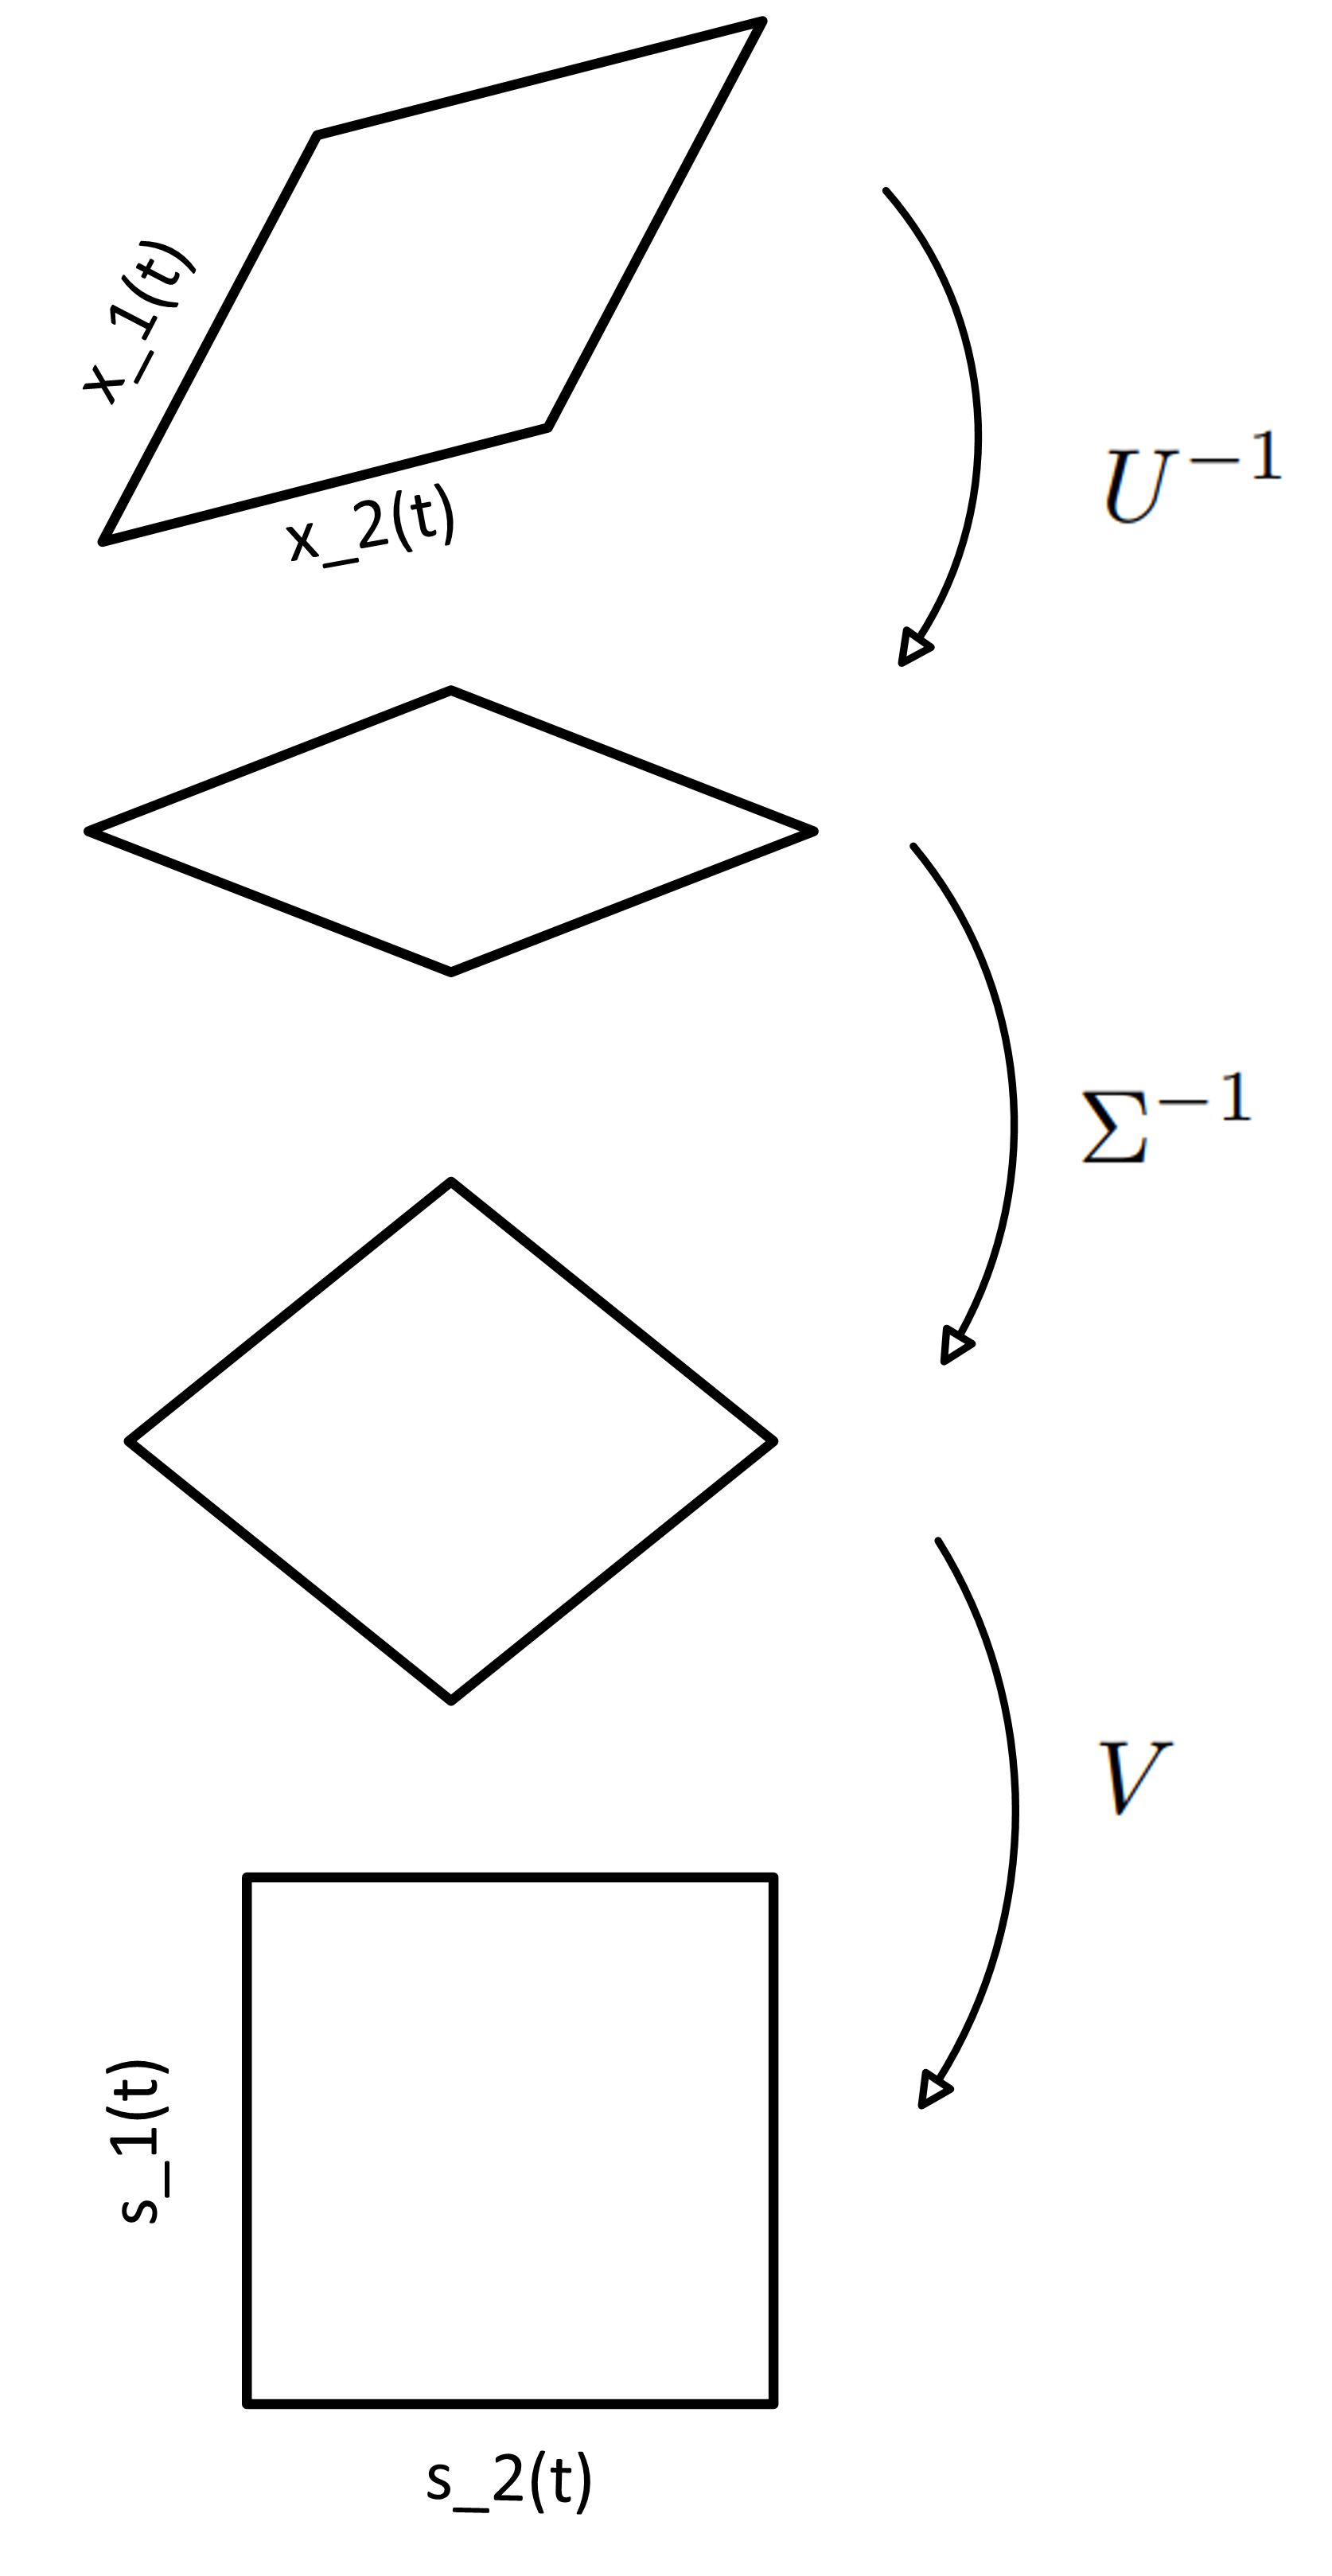
\includegraphics[height=6.5cm, width=0.35\textwidth]{figuras/ICA/ICA_geometry.png}
    \caption{Geometric interpretation of ICA in the 2D case. The observed mixtures are decorrelated with PCA (first step) and normalized (second step). Once the data is whitened the final step corresponds to the rotation that best recovers the statistically independent sources.} 
    \label{fig:ica_geometry}
\end{figure}

\section{Implementations: FastICA}
\label{sec:ica_implementation}


Although the ICA framework provides a clear approach for separating mixed sources, obtaining the final separation matrix is not trivial. The algorithm relies on finding the projection directions that maximize the non-Gaussianity of the estimated sources, which can result computationally expensive if performed directly through kurtosis maximization. Therefore, this section focuses on \textbf{FastICA} \cite{scikit-learn_scikit-learnsklearndecomposition_fasticapy_nodate}, one of the most practical implementations of ICA. Even though this algorithm is already available in libraries, reviewing its steps is useful to later introduce the modified algorithm for constrained ICA (chapter \ref{ch:constrained_ica})
. 

FastICA relies on \textbf{fixed-point iteration}, which updates an initial guess repeatedly until the result stops significantly changing. This initial guess is a randomized separation direction, which is constantly corrected by the algorithm until it stabilizes. Equation \ref{eq:fixed_point} shows the general form of this fixed-point update, where each new estimate $w^{(k+1)}$ is obtained by applying the update function $F(\cdot)$ to the previous estimate $w^{(k)}$ until $w^{(k+1)}$ and $w^{(k)}$ become similar.

\begin{equation}
    \mathbf{w}^{(k+1)} = F(\mathbf{w}^{(k)})
    \label{eq:fixed_point}
\end{equation}


Additionally, FastICA mainly uses \textbf{negentropy} as the measure of non-Gaussianity, since it is more robust than directly maximizing kurtosis. Negentropy essentially measures how far a random variable is from a Gaussian distribution, being zero for a Gaussian variable and positive for non-Gaussian variables. In practice, it is not calculated directly, but approximated using nonlinear contrast functions like in Equation \ref{eq:negentropy_approx}.
\begin{equation}
    J(y) \propto
\left[
\mathbb{E}\{G(y)\}
-
\mathbb{E}\{G(v)\}
\right]^2
\label{eq:negentropy_approx}
\end{equation}
where \(v\) is a standard Gaussian variable and \(G(\cdot)\) is a chosen nonlinear function. Since $\mathbb{E}\{G(v)\}$ is constant in this problem, the optimization focuses on estimation $y$. In FastICA, $y$ is the estimated component, so in this context $\mathbf{y=w^T z}$. Taking this into account, the update rule (\ref{eq:fixed_point}) is derived from the negentropy approximation (\ref{eq:negentropy_approx}) under the unit-norm constraint.\footnote{This constraint ($|| \mathbf{w}||^2$ = 1) fixes arbitrary scale and bounds feasible region for the maximization problem.} Equation \ref{eq:update_step} shows the update step where the constraint is imposed through a Lagrange multiplier.\footnote{Lagrange multiplier: $\mathcal{L}(w,\lambda)=g(x)-\lambda f(x)$ in this case is the constraint $f(x)=||w||^2-1$}

\begin{equation}
    \mathbf{w}^{(k+1)}
=
\mathbb{E}\left\{
\mathbf{z}\, g\left(\mathbf{w}^{(k)T}\mathbf{z}\right)
\right\}
-
\lambda \mathbf{w}^{(k)}, \qquad 
\lambda =
\mathbb{E}\left\{
g'\left(\mathbf{w}^{(k)T}\mathbf{z}\right)
\right\} 
\label{eq:update_step}
\end{equation}
 

\noindent Once fixed-point iteration is understood, FastICA can be summarized as three main steps:

\begin{enumerate}
    \item \textbf{Preprocess the observations:} the EMG matrix is centered and whitened so that second-order dependencies are removed (already addressed in chapter \ref{ch:preprocessing}).
    
    \item \textbf{Update fixed-point iteration:} the algorithm applies a fixed-point update that searches for maximally non-Gaussian projections.
    
    \item \textbf{Ensure orthogonality and convergence:} after each update, symmetric decorrelation is applied and the change in the separation vectors is evaluated.
\end{enumerate}

Listing \ref{lst:fastica_pseudocode} shows the general implementation structure followed in this work. the line \texttt{FixedPointUpdate}(W, Z, g) represents the update in Equation \ref{eq:update_step}, while \texttt{SymmetricDecorrelate(W)} ensures that the estimated components remain orthogonal.

\begin{lstlisting}[
style=pseudocode,
caption={FastICA algorithm pseudocode},
label={lst:fastica_pseudocode}
]
Input: Observed EMG matrix X, number of components K,
       tolerance epsilon, maximum iterations Imax

Output: Estimated sources S_hat and separation matrix W

//Preprocessing
Xc <- X - mean(X)
Z  <- Whiten(Xc)
//Iniziatilation
W <- RandomInitialization(K)
W <- SymmetricDecorrelate(W)

//Negentropy optimization
for i = 1 to Imax

    W_old <- W
    W <- FixedPointUpdate(W, Z, g)
    W <- SymmetricDecorrelate(W)
    delta <- max_j | |w_j * w_old_j^T| - 1 |

    if delta < epsilon
        break
    end
    
end

S_hat <- Xc * W^T

return S_hat, W
\end{lstlisting}

Overall, the main advantage of this implementation is that the optimization is reduced to repeated matrix updates. This makes FastICA suitable as a practical baseline method for the EMG separation experiments, where several noise levels and mixing conditions must be evaluated.
\clearpage

\section{Weak-source and noise}
\label{sec:weak_source_and_noise}

In the context of this study, one of the main difficulties does not come only from the mixing itself, but from the fact that the target component may be significantly weaker than the interfering source. Under noisy conditions, source separation becomes more challenging, since the contribution of the weaker signal to the observed mixtures may be partially masked by both the dominant component and the additive noise. For this reason, it is crucial to analyze how weak-source conditions and noise affect the identifiability and practical recovery of the signals \cite{naik_blind_2014}.
\subsection{Instantaneous mixtures}
Consider the instantaneous ($\mathbf{\tau=0}$ ms) noisy mixing model
\begin{equation}
\mathbf{x}=\mathbf{A}\mathbf{s}+\mathbf{n},
\qquad
\mathbf{A}=
\begin{bmatrix}
a_{11} & a_{12}\\
a_{21} & a_{22}
\end{bmatrix},
\label{eq:weak_noise_model}
\end{equation}
where $\mathbf{n}$ denotes an additive noise vector. In the noiseless case, the presence of a weak source does not theoretically prevent exact recovery as long as the mixing matrix is invertible ($det(A)=a_{11}a_{22}-a_{12}a_{21} \neq0$). Therefore, the main difficulty does not arise from the amplitude asymmetry alone, but from the way in which additive noise is transformed by the inverse mixing matrix.

Applying the ideal inverse transformation to \eqref{eq:weak_noise_model} yields
\begin{equation}
\hat{\mathbf{s}}=\mathbf{A}^{-1}\mathbf{x}
=\mathbf{A}^{-1}(\mathbf{A}\mathbf{s}+\mathbf{n})
=\mathbf{s}+\mathbf{A}^{-1}\mathbf{n}.
\label{eq:inverse_noise_general}
\end{equation}
Therefore, even if the sources are theoretically separable, the recovered signal is affected by a noise term transformed by the inverse mixing matrix. This means that the practical difficulty of the recovery problem depends not only on the source amplitudes, but also on how $\mathbf{A}^{-1}$ amplifies the additive perturbations.

For a general $2\times 2$ mixing matrix, the inverse can be written as
\begin{equation}
\mathbf{A}^{-1}
=
\frac{1}{a_{11}a_{22}-a_{12}a_{21}}
\begin{bmatrix}
a_{22} & -a_{12}\\
-a_{21} & a_{11}
\end{bmatrix}
\label{eq:inverse_A_general}
\end{equation}
provided that $\det(\mathbf{A})=a_{11}a_{22}-a_{12}a_{21}\neq 0$. 
If the objective is to recover the first source, the corresponding estimation error is given by the first component of $\mathbf{A}^{-1}\mathbf{n}$, namely
\begin{equation}
e_1=
\frac{1}{a_{11}a_{22}-a_{12}a_{21}}
\left(a_{22}n_1-a_{12}n_2\right).
\label{eq:e1_general}
\end{equation}Therefore, its variance can be written as
\begin{equation}
\mathrm{Var}(e_1)=
\frac{
a_{22}^2\mathrm{Var}(n_1)
+a_{12}^2\mathrm{Var}(n_2)
-2a_{22}a_{12}\mathrm{Cov}(n_1,n_2)
}{
\left(a_{11}a_{22}-a_{12}a_{21}\right)^2
}.
\label{eq:var_e1_expanded}
\end{equation}
Assuming that $n_1$ and $n_2$ are zero-mean, uncorrelated and have equal variance $\sigma^2$, the variance of this error (and similarly $e_2$) becomes
\begin{equation}
\mathrm{Var}(e_1)=
\frac{\sigma^2\left(a_{22}^2+a_{12}^2\right)}
{\left(a_{11}a_{22}-a_{12}a_{21}\right)^2} \qquad
\mathrm{Var}(e_2)=
\frac{\sigma^2\left(a_{12}^2+a_{11}^2\right)}
{\left(a_{11}a_{22}-a_{12}a_{21}\right)^2}
\label{eq:var_e1_e2_general}
\end{equation}

From equation \eqref{eq:inverse_noise_general}, the recovered sources can be written as
\begin{equation}
\hat{s}_1 = s_1 + e_1 \qquad
\hat{s}_2 = s_2 + e_2
\label{eq:s1s2_hat_error}
\end{equation}
where $e_1,e_2$ are the error terms introduced by the transformed noise. This expression allows the previous result to be connected with two practical performance measures: the output SNR and the correlation between the true and recovered sources.
Assuming that $e_1$ is uncorrelated with $s_1$, the output SNR for the first recovered source can be defined as
\begin{equation}
\mathrm{SNR}_1=\frac{\mathrm{Var}(s_1)}{\mathrm{Var}(e_1)}
\label{eq:snr1_def}
\end{equation}
Similarly, using \eqref{eq:s1s2_hat_error} and the assumption that $s_1$ and $e_1$ are uncorrelated, the correlation between $s_1$ and $\hat{s}_1$ can be written as
\begin{equation}
\rho_{s_1,\hat{s}_1}=
\frac{\mathrm{Cov}(s_1,\hat{s}_1)}
{\sqrt{\mathrm{Var}(s_1)\mathrm{Var}(\hat{s}_1)}} = \frac{1}{\sqrt{1+\frac{\mathrm{Var}(e_1)}{\mathrm{Var}(s_1)}}}
\label{eq:corr_def}
\end{equation}

The previous derivation provides general expressions for the output correlation and SNR by describing how additive noise propagates through the inverse mixing matrix $A^{-1}$ and affects the recovered sources. It is worth noting that as $\mathbf{det(A)}$ approaches 0, both error variances grow rapidly. Given the equations \ref{eq:snr1_def} and \ref{eq:corr_def}, greater values of $\mathrm{Var}(e_1)$ and  $\mathrm{Var}(e_2)$ worsen the SNR and correlation, \uline{ which implies that noise has a greater effect on the separation when $\mathbf{det(A)}\rightarrow 0$. } This can be seen in Figure \ref{fig:det_0}, which  shows the separation quality graph for different values of the determinant of the mixing matrix A in \textbf{symmetric attenuation scenario (model in \ref{sec:symmetric_attenuation})}.

\begin{figure}[H]
    \centering
    \makebox[\textwidth][c]{%
        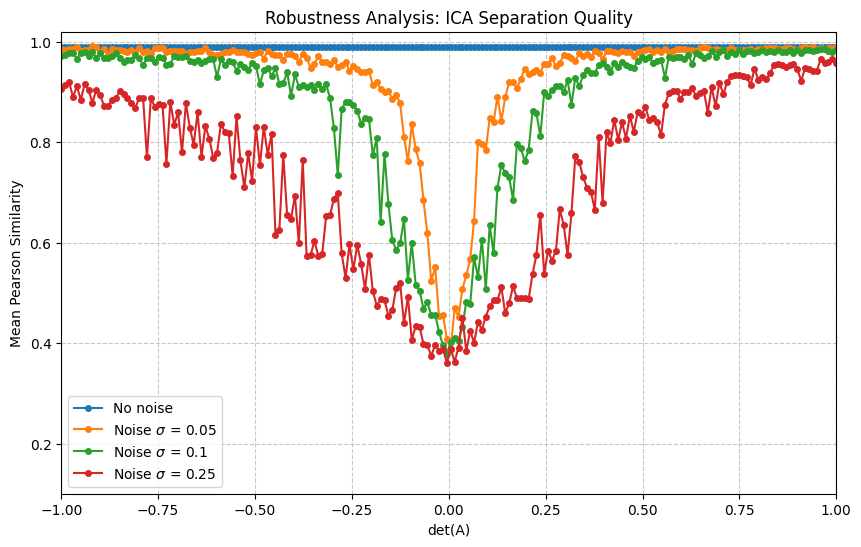
\includegraphics[width=\linewidth, height=8.5cm]{figuras/ICA/det_close_to_0.png}
    }
    \caption{Robustness analysis: how the determinant values affect the mean correlation of the estimations $\hat{s}_1$ and $\hat{s}_2$ with the original sources $s_1$ and $s_2$ (\textbf{symmetrical attenuation case}).}
    \label{fig:det_0}
\end{figure}


Additionally, to relate these results to the specific problem addressed in this work, it is useful to consider these metrics under the model described in section \ref{sec:weak_source_regime}, where $\mathbf{a_{11}=a_{22}=1 \gg a_{21}}$ and $\mathbf{a_{12}=\beta \in[0,1]}$. This substitution makes it easier to specifically explain how the parameter $\beta$ influences the recovery of the weak target source. Consequently, the corresponding output SNR and source-estimate correlation can also be written as functions of $\beta$.

\begin{equation}
\rho_{s_1,\hat{s}_1}
 = \frac{1}{\sqrt{1+\frac{\sigma^2 (1+\beta^2)}{\mathrm{Var}(s1)}}}
 \qquad
 \mathrm{SNR}_1=\frac{\mathrm{Var}(s1)}{\sigma^2 (1+\beta^2)} \qquad \beta \in[0,1]
\label{eq:s1_metrics_with_beta}
\end{equation}

\begin{equation}
\rho_{s_2,\hat{s}_2}
 = \frac{1}{\sqrt{1+\frac{\sigma^2}{\mathrm{Var}(s2)}}}
 \qquad
 \mathrm{SNR}_2=\frac{\mathrm{Var}(s2)}{\sigma^2} \qquad \beta \in[0,1]
\label{eq:s2_metrics_with_beta}
\end{equation}

Given these expressions, it is easier to draw explicit conclusions about the influence of the parameter $\beta$ over the separation process. Equation \ref{eq:s1_metrics_with_beta} demonstrates that the estimation of $s1$ (weak source) is worsened as $\beta$ increases, since $\mathrm{SNR}_1 \propto \frac{1}{1+\beta^2}$, but by much since in this case $\beta$ is bounded to $[0, 1]$. This can also be explained by the distance.However, the dominant signal (in this case $s_2$) is theoretically not affected by the $\beta$ parameter as it does not appear in the correlation and SNR expressions for $s_2$. Figures \ref{fig:beta_effect_s1_corr_weak_source} and \ref{fig:beta_effect_s1_snr_weak_source} graphically show how correlation and SNR of the estimated $s_1$ are affected by $\beta$ in this case, but \uline{numerical values also depend on $\mathrm{Var}(s1)$}.

\begin{figure}[H]
    \centering
    \makebox[\textwidth][c]{%
        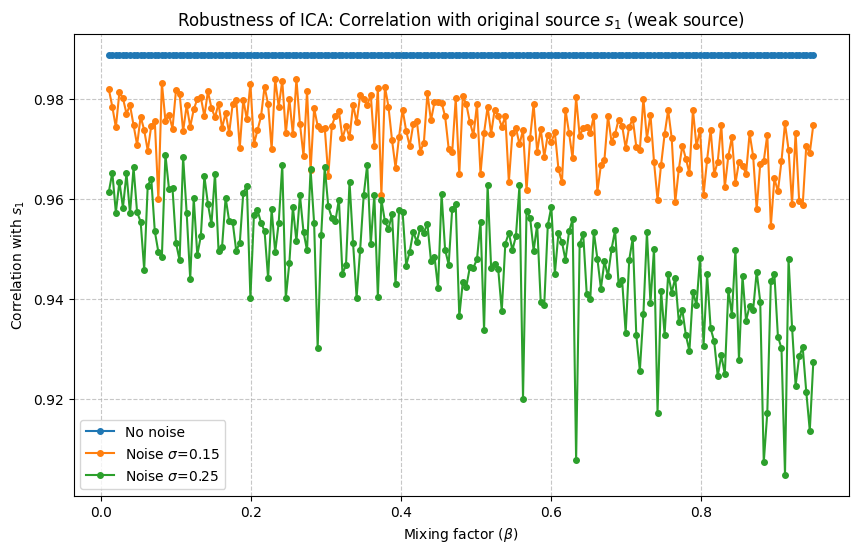
\includegraphics[width=\linewidth]{figuras/ICA/beta_effect_s1_corr_weak_source.png}
    }
    \caption{Robustness analysis: correlation of $\hat{s}_1$ with original source $s_1$ considering the weak source model (Section \ref{sec:weak_source_regime}).}
    \label{fig:beta_effect_s1_corr_weak_source}
\end{figure}

\begin{figure}[H]
    \centering
    \makebox[\textwidth][c]{%
        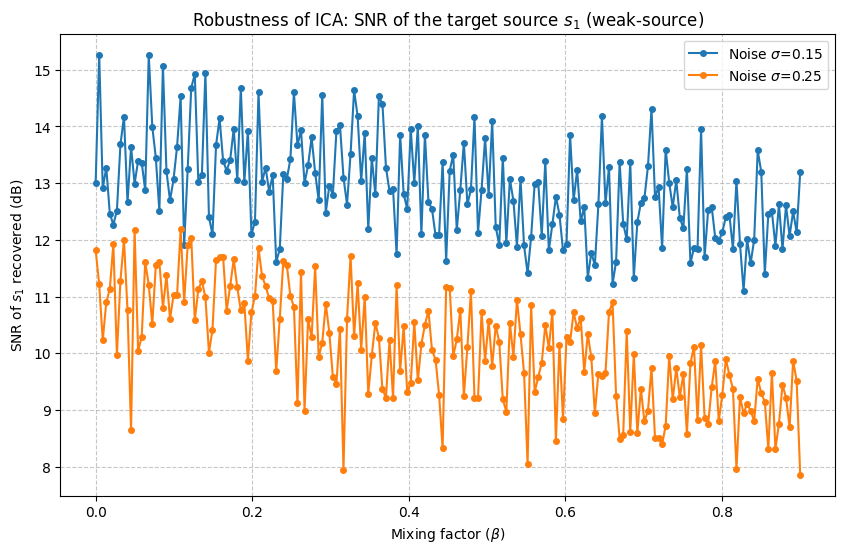
\includegraphics[width=\linewidth, height=8.5cm]{figuras/ICA/beta_effect_s1_snr_weak_source.png}
    }
    \caption{Robustness analysis: SNR of $\hat{s}_1$ considering the weak source model (Section \ref{sec:weak_source_regime}).}
    \label{fig:beta_effect_s1_snr_weak_source}
\end{figure}

Nevertheless, it is worth noting that in symmetric attenuation (model \ref{sec:symmetric_attenuation}), this  influence is greater as  $\beta \in [0,1)$ causes $det(a)$ to approach 0. Figures \ref{fig:beta_effect_s1_corr} and \ref{fig:beta_effect_s1_snr} show correlation and SNR for the estimated $s_1$ in this case.

\begin{figure}[H]
    \centering
    \makebox[\textwidth][c]{%
        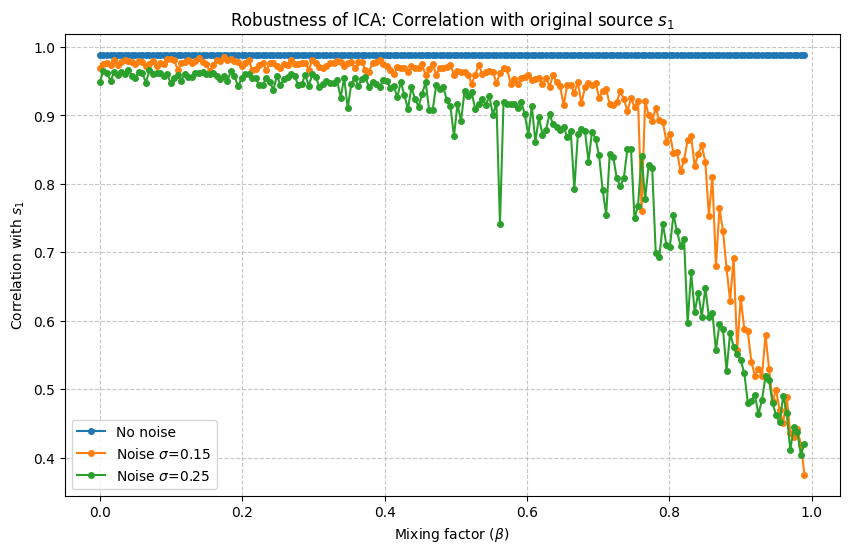
\includegraphics[width=\linewidth, height=8.5cm]{figuras/ICA/beta_effect_s1_corr.png}
    }
    \caption{Robustness analysis: correlation of $\hat{s}_1$ with original source $s_1$ considering the symmetric attenuation model (Section \ref{sec:symmetric_attenuation})}
    \label{fig:beta_effect_s1_corr}
\end{figure}

\begin{figure}[H]
    \centering
    \makebox[\textwidth][c]{%
        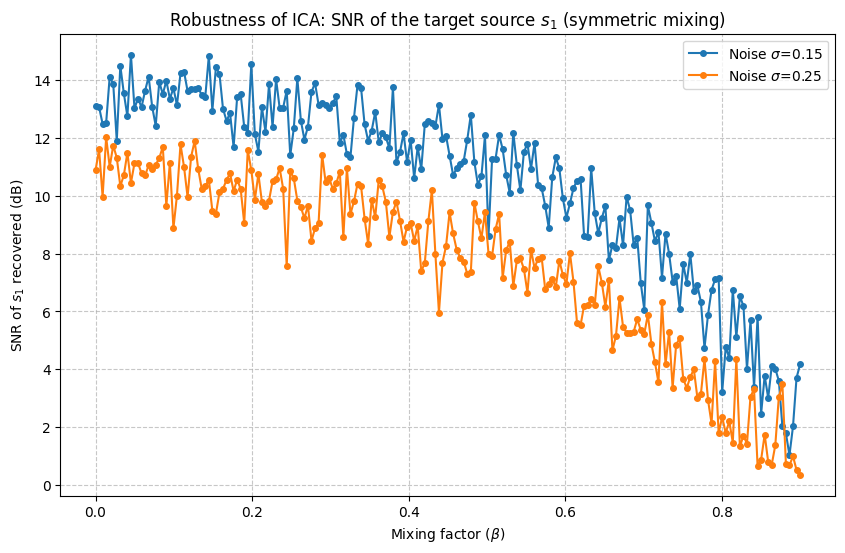
\includegraphics[width=\linewidth]{figuras/ICA/beta_effect_s1_snr.png}
    }
    \caption{Robustness analysis: SNR of $\hat{s}_1$ considering the symmetric attenuation model (Section \ref{sec:symmetric_attenuation}).}
    \label{fig:beta_effect_s1_snr}
\end{figure}

Overall, noise plays an important role in source separation, especially if the mixing matrix $\mathbf{A}$ is close to being singular. This  effect is especially relevant in the symmetric attenuation model (Section \ref{sec:symmetric_attenuation}), where $\beta \in [0,1)$ is closer to singular matrix. By contrast, in the weak source regime (Section \ref{sec:weak_source_regime}) this issue is less important with $\beta \in [0,1]$, since $det(A)=0$ would only occur at $\beta=100$. Therefore, in this model, the main limitation is the dominance of the stronger source over the weak target source, rather than the effect of noise alone.

\subsection{Convolutive mixtures}
\label{subsec:conv_mixtures}

The previous analysis assumes an instantenous mixing model, which makes it possible to describe the separation process through a fixed constant mixing matrix. This makes it simple to derive closed-form expressions for the noise influence, the output SNR of each original signal and the source-estimate correlation. However, when delay is introduced, these assumptions no longer hold and the expressions derived in the previous section do not apply directly \cite{brendel_unifying_2023}.

More specifically, if each sources reach the observed channels with a relative delay, denoted as $\tau$, the model becomes convolutive. Let $D_\tau$ be the delay operator, defined as $D_\tau x(t)=x(t-\tau).$ Then the delayed mixing model can be expressed as 

\begin{equation}
    \mathbf{x}(t)=\mathbf{A}_{\tau}\mathbf{s}(t)+\mathbf{n}(t),
    \qquad
    \mathbf{A}_{\tau}=
    \begin{bmatrix}
    a_{11} & a_{12}D_{\tau}\\
    a_{21}D_{\tau} & a_{22}
    \end{bmatrix}
\label{eq:conv_matrix_model}
\end{equation}

\clearpage

For a conventional instantaneous FastICA model, the main problem is that the demixing matrix is
assumed to be constant. Therefore, delayed contributions cannot be perfectly
cancelled by an instantaneous inverse. In this case, the delayed source term
acts as a residual interference component \cite{parra_convolutive_2000}.

Let $r_{s_2}(\tau)$ express the normalized autocorrelation of the dominant source
$s_2$ at lag $\tau$,

\begin{equation}
r_{s_2}(\tau)=
\frac{\mathbb{E}\{s_2(t)s_2(t-\tau)\}}
{\operatorname{Var}(s_2)}
\end{equation}
If an instantaneous model tries to approximate the delayed term $s_2(t-\tau)$
from the non-delayed signal $s_2(t)$, the best linear approximation is

\begin{equation}
s_2(t-\tau) \approx r_{s_2}(\tau)s_2(t)
\end{equation} The part that cannot be represented by the instantaneous model is therefore

\begin{equation}
e_\tau(t)=s_2(t-\tau)-r_{s_2}(\tau)s_2(t)
\end{equation}
Assuming $s_2$ is zero-mean, its residual power becomes

\begin{equation}
\begin{aligned}
P_{\mathrm{res}}(\tau)
&= \beta^2 \operatorname{Var}(e_\tau)
= \beta^2 \operatorname{Var}(s_2)
\left(1-r_{s_2}^2(\tau)\right)
\end{aligned}
\end{equation}Consequently, the effective SNR of the estimated weak source can be approximated as

\begin{equation}
\operatorname{SNR}_{1,\tau}
\approx
\frac{\operatorname{Var}(s_1)}
{\sigma^2+
\beta^2 \operatorname{Var}(s_2)
\left(1-r_{s_2}^2(\tau)\right)}
\label{eq:delay_contamination_term}
\end{equation}

This expression shows that, when $\tau \approx 0$, then
$r_{s_2}(\tau)\approx 1$ and the delayed model behaves similarly to the
instantaneous case. Theoretically, if $\tau$ increases, $r_{s_2}(\tau)$ should decrease, the interference increase and the SNR of the weak source estimation be affected. However, this behavior mainly depends on the autocorrelation function, which can make the interference term oscillate in some regions, as shown in Table \ref{tab:autocorr_residual_tau}. 

\begin{table}[H]
\centering


\begin{tabular}{c|c|c|c}
\hline
$\tau$ & $r_{s_2}(\tau)$ & $r_{s_2}^2(\tau)$ & $1-r_{s_2}^2(\tau)$ \\
\hline
1  &  0.522 & 0.273 & 0.727 \\
2  & -0.259 & 0.067 & 0.933 \\
3  & -0.493 & 0.243 & 0.757 \\
4  & -0.284 & 0.081 & 0.919 \\
5  & -0.106 & 0.011 & 0.989 \\
6  & -0.046 & 0.002 & 0.998 \\
10 &  0.087 & 0.008 & 0.992 \\
\hline
\end{tabular}
\caption{Normalized autocorrelation values of $s_2$ and corresponding residual factor.}
\label{tab:autocorr_residual_tau}
\end{table}

\clearpage


\section{Scale reconstruction}
\label{sec:scale_reconstruction}
As mention in Section \ref{sec:ica_problem_formulation}, one limitation of ICA source separation is the scale indetermination of the recovered sources. Even if the estimated sources have the correct waveform, their amplitudes are often not the same. Therefore, denormalization (due to preprocessing stage) and an additional scaling step is required to obtain source estimates with amplitudes consistent with the observed mixtures.

In this work, for the scale reconstruction, negligible noise is assumed  for simplification. This is done because the noise power cannot be reliably estimated from the available mixtures. For this reason, the resulting scale factors should be interpreted as approximate amplitude corrections. It is worth noting that this scaling step is not included in the experiments presented in this thesis. However, it is an important factor that should be considered in real world testing, where the amplitude of the recovered sources may be relevant for EMG detection.


This scale reconstruction can be estimated using either RMS or variance values,
since both statistics are directly related for zero-mean signals. This relation
is shown in Equation~\ref{eq:rms_definition}.

\begin{equation}
\mathrm{RMS}^2(x)
=
\frac{1}{N}\sum_{n=1}^{N}x[n]^2
=
\operatorname{Var}(x)
\qquad \text{if } \mathbb{E}[x]=0
\label{eq:rms_definition}
\end{equation}

For the asymmetric two-source mixture considered in this work, the observed channels are modeled as shown in Equations \ref{eq:scale_mixture_c1} and \ref{eq:scale_mixture_c2}, which are discrete representations of the model studied in this thesis.

\begin{equation}
c_1[n]=s_1[n]+\beta s_2[n]
\label{eq:scale_mixture_c1}
\end{equation}

\begin{equation}
c_2[n]=0.01s_1[n]+s_2[n]
\label{eq:scale_mixture_c2}
\end{equation}
where $\beta$ controls the interference of $s_2$ into the first channel and $0.01$ represents a weak contribution of $s_1$ into the second channel. From \ref{eq:scale_mixture_c1}, the squared RMS of the first channel can be written as 

\begin{equation}
\mathrm{RMS}^2(c_1)
=
\mathrm{RMS}^2(s_1)
+
\beta^2\mathrm{RMS}^2(s_2)
+
2\beta\operatorname{Cov}(s_1,s_2)
\label{eq:rms_c1_full}
\end{equation}

Assuming that $s_1$ and $s_2$ are independent and approximately zero-mean, the \textbf{covariance term is approximately zero}. Since the recovered ICA sources are affected by an arbitrary scale factor, the true sources can be related to the estimated sources as

\begin{equation}
\mathrm{RMS}(s_i)=\alpha_i\mathrm{RMS}(\hat{s}_i)
\qquad i=1,2
\label{eq:scale_factor_definition}
\end{equation}
where $\alpha_i$ is the scale reconstruction factor of source $i$. Substituting \ref{eq:scale_factor_definition} into the RMS relations gives a system of two variables ($\alpha_1$ and $\alpha_2$).

\begin{equation}
\left\{
\begin{aligned}
\mathrm{RMS}^2(c_1)
&\approx
\alpha_1^2\mathrm{RMS}^2(\hat{s}_1)
+
\beta^2\alpha_2^2\mathrm{RMS}^2(\hat{s}_2)
\\[0.4em]
\mathrm{RMS}^2(c_2)
&\approx
0.01^2\alpha_1^2\mathrm{RMS}^2(\hat{s}_1)
+
\alpha_2^2\mathrm{RMS}^2(\hat{s}_2)
\end{aligned}
\right.
\label{eq:rms_scaled_system}
\end{equation}
\\
Solving the system in \ref{eq:rms_scaled_system} for the scale factor of the first source yields

\begin{equation}
\alpha_1(\beta)
=
\sqrt{
\frac{
\mathrm{RMS}^2(c_1)
-
\beta^2\mathrm{RMS}^2(c_2)
}
{
\mathrm{RMS}^2(\hat{s}_1)\left(1-0.01^2\beta^2\right)
}
}
\label{eq:alpha1_beta}
\end{equation}

Similarly, the scale factor of the second source can be obtained as shown in Equation \ref{eq:alpha2_beta}

\begin{equation}
\alpha_2(\beta)
=
\sqrt{
\frac{
\mathrm{RMS}^2(c_2)
-
0.01^2\mathrm{RMS}^2(c_1)
}
{
\mathrm{RMS}^2(\hat{s}_2)\left(1-0.01^2\beta^2\right)
}
}
\approx
\sqrt{
\frac{
\mathrm{RMS}^2(c_2)
}
{
\mathrm{RMS}^2(\hat{s}_2)
}
}
\label{eq:alpha2_beta}
\end{equation}

The approximation in \ref{eq:alpha2_beta} is justified by the fact that $0.01^2$ is very small, so the contribution of $s_1$ to the energy of $c_2$ is negligible. Equations \ref{eq:alpha1_beta} and \ref{eq:alpha2_beta} provide an approximate reconstruction of the source amplitudes from the observed channel energies, assuming that the mixing coefficients are known or controlled.

If a temporal delay is introduced in the cross-talk terms, like in Equations \ref{eq:delayed_c1} and \ref{eq:delayed_c2}, then the RMS-based derivation remains approximately valid.

\begin{equation}
c_1[n]=s_1[n]+\beta s_2[n-\tau]
\label{eq:delayed_c1}
\end{equation}

\begin{equation}
c_2[n]=0.01s_1[n-\tau]+s_2[n]
\label{eq:delayed_c2}
\end{equation}
This is because a time shift
does not significantly change the signal energy when boundary effects are
negligible. 

\begin{equation}
\mathrm{RMS}^2(x[n-\tau]) \approx \mathrm{RMS}^2(x[n])
\qquad \tau \ll N
\label{eq:rms_delay_approx}
\end{equation}

For finite length EMG windows, a delay implemented with zero-padding may slightly
alter the RMS value because samples at the boundaries lost or replaced by
zeros. However, when the delay is small compared to the window length, this
effect is negligible. Therefore, the reconstruction in
\ref{eq:alpha1_beta} and \ref{eq:alpha2_beta} remains approximately unchanged under the assumption that boundary effects are negligible.

An additional final note is that this scale factor estimation is not specific to ICA. The same rescaling procedure can be applied to the other separation
algorithms considered in this thesis, since the recovered components also
present arbitrary amplitude scales.
\clearpage

\section{ICA results}

Up to this point, this chapter has focused on explaining the theoretical considerations of ICA for all the proposed models. However, this final ICA section aims to test the performance of the algorithm for the case of the IIT study (model \ref{eq:2d_beta_asymmetric_system}) on possible scenarios. The goal is not to recover the exact waveform of the target-flap related source ($s_1$), but to preserve its activations and behavior as accurately as possible. In these results, the main metric of interest is $corr_{rms}(\hat{s}_1,s1)$, which represents the correlation of the RMS envelopes of the estimated source $\hat{s}_1$ and $s_1$. For these experiments, $\mathbf{\beta=0.9}$ is assumed unless mentioned otherwise.

\subsection{Ideal case}
\label{subsec:ica_experiment_ideal}

This case shows ICA performance when all of its main assumptions are satisfied. Figure \ref{fig:ica_result_ideal} shows how the muscle signals $s_1$ and $s_2$ are recovered. The separation achieves perfect temporal and RMS envelope correlation, but, as mention in Section \ref{sec:ica_problem_formulation}, \uline{the order and scale of the signals is lost}. However, these two aspects can be easily addressed: 

\begin{itemize}
    \item \textbf{Order:} permutation does not result in a problem in this model. Since mixture $c_2 \approx s_2$, $s_1$ is simply the orthogonal direction.
    \item \textbf{Scale:} not critical as long as the recovered component remains correlated with the target source. 
\end{itemize}
 

\begin{figure}[H]
    \centering
    \makebox[\textwidth][c]{%
        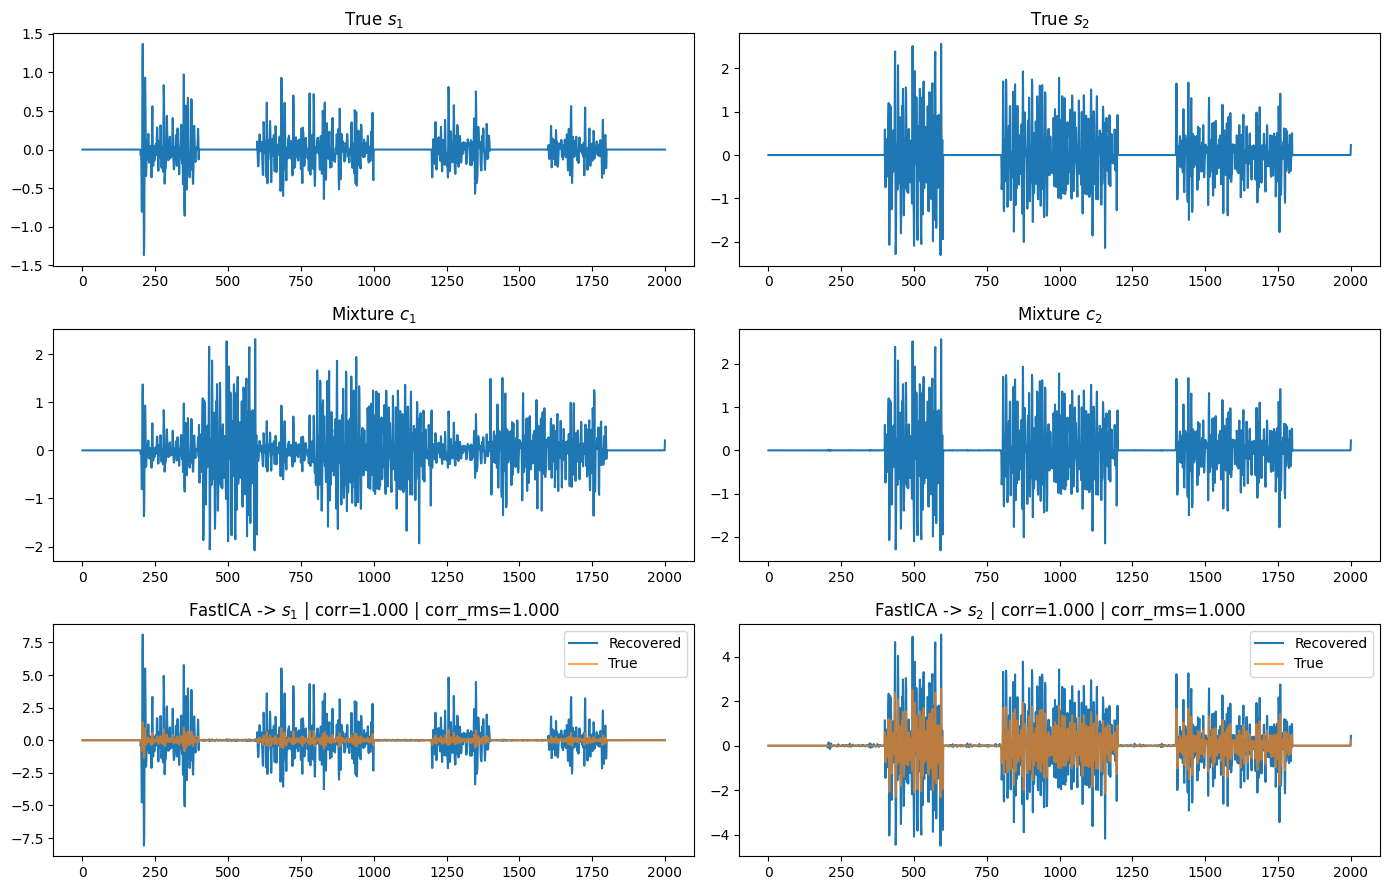
\includegraphics[width=\linewidth]{figuras/ICA/ica_result_ideal.png}
    }
    \caption{Ideal case. FastICA recovers both sources with perfect correlations, but suffers from the expected scale ambiguity. The estimation and the original source may have different amplitudes, but both signals behave the same.}
    \label{fig:ica_result_ideal}
\end{figure}
\subsection{Instantaneous mix with noise}
\label{subsec:ica_experiment_noise}

This case maintains all simulation variables from previous section, but adds additive white gaussian noise with variance $\sigma^2$. Since the signals are normalized, $\sigma=0.1$ and $\sigma=0.15$ can be considered as relative noise levels. This consistent with EMG methodology reports suggesting that differences in detection conditions can introduce around 10\% to 15\% variability in repeated measurements \cite{konrad_abc_2005}. For this reason, the experiments were run with \uline{$\sigma=0.1$} for simplification.

Figure \ref{fig:ica_result_noise} shows that the estimation $s_1$ has a worse temporal correlation with its original source, but maintains a remarkable RMS envelope correlation. This can be explained as small waverform errors directly impact temporal correlation while activation patterns are maintained. By contrast, $s_2$ is less affected by noise due to two main reasons:

\begin{itemize}
    \item \textbf{Dominance in the mixing model:} as established in Equation \ref{eq:s2_metrics_with_beta}, $\rho_{s_2,\hat{s}_2}$ and $\mathrm{SNR}_2$ do not depend on the $\beta$ parameter.
    \item $\mathbf{\mathrm{Var}(s_2)>>\mathrm{Var}(s_1),\mathrm{Var}(n)}$\textbf{:} in this case the noise variance negligible compared to $s_2$, but not for $s_1$.
\end{itemize}

It is also worth noting that, even though the values of $\beta$ and $\sigma$ are fixed, $corr(\hat{s}_1,s_1)$ and $corr_{rms}(\hat{s}_1,s_1)$ still depend on $\mathrm{Var}(s_1)$. 


\begin{figure}[H]
    \centering
    \makebox[\textwidth][c]{%
        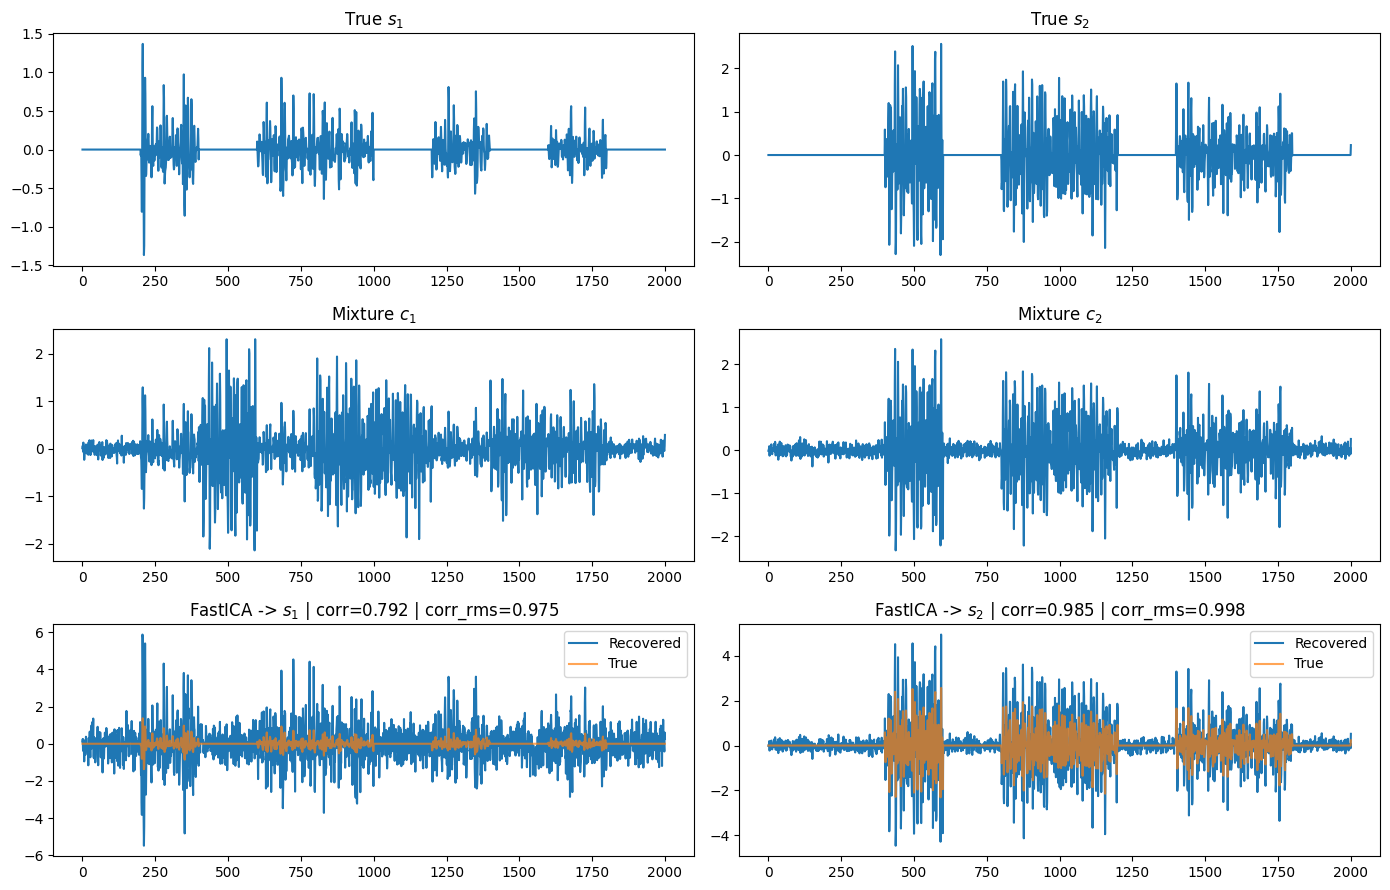
\includegraphics[width=\linewidth]{figuras/ICA/ica_result_noise.png}
    }
    \caption{Separation under noisy instantaneous mixing. Parameters were set to $\sigma=0.1$, $\beta=0.9$ and $\tau=\qty{0}{ms}$. FastICA struggles to maintain temporal correlation with $s_1$, but recovers activation patterns. }
    \label{fig:ica_result_noise}
\end{figure}
\clearpage
\subsection{Convolutive mixture with noise}

This final scenario adds to the previous instantaneous noisy mixture by including delay between EMG sources, making it a convolutional mixture problem. As mentioned in Section \ref{subsec:conv_mixtures}, FastICA's quality of separation is degraded by the presence of a delay $\mathbf{\tau}$, which makes the recovery of the weak source $s_1$ dependent on the dominant signals autocorrelation $\mathbf{r_{s_2}(\tau)}$. For this experiment, \uline{$\tau=5$ ms} is set to accurately relate to a real world scenario \cite{muceli_tutorial_2024}. 

Compared to previous cases, Figure \ref{fig:ica_result_noise_delay09} shows that the estimation $\hat{s}_1$ for $s_1$ has a noticeably lower temporal correlation and significantly worse correlation with the original RMS envelope. This points to the delayed interference term (Equation \ref{eq:delay_contamination_term}) drastically impacting the structure of the signal. However, it can be noticed that the estimation for $s_2$ remains optimal due to the factors mentioned throughout the chapter. 


\begin{figure}[H]
    \centering
    \makebox[\textwidth][c]{%
        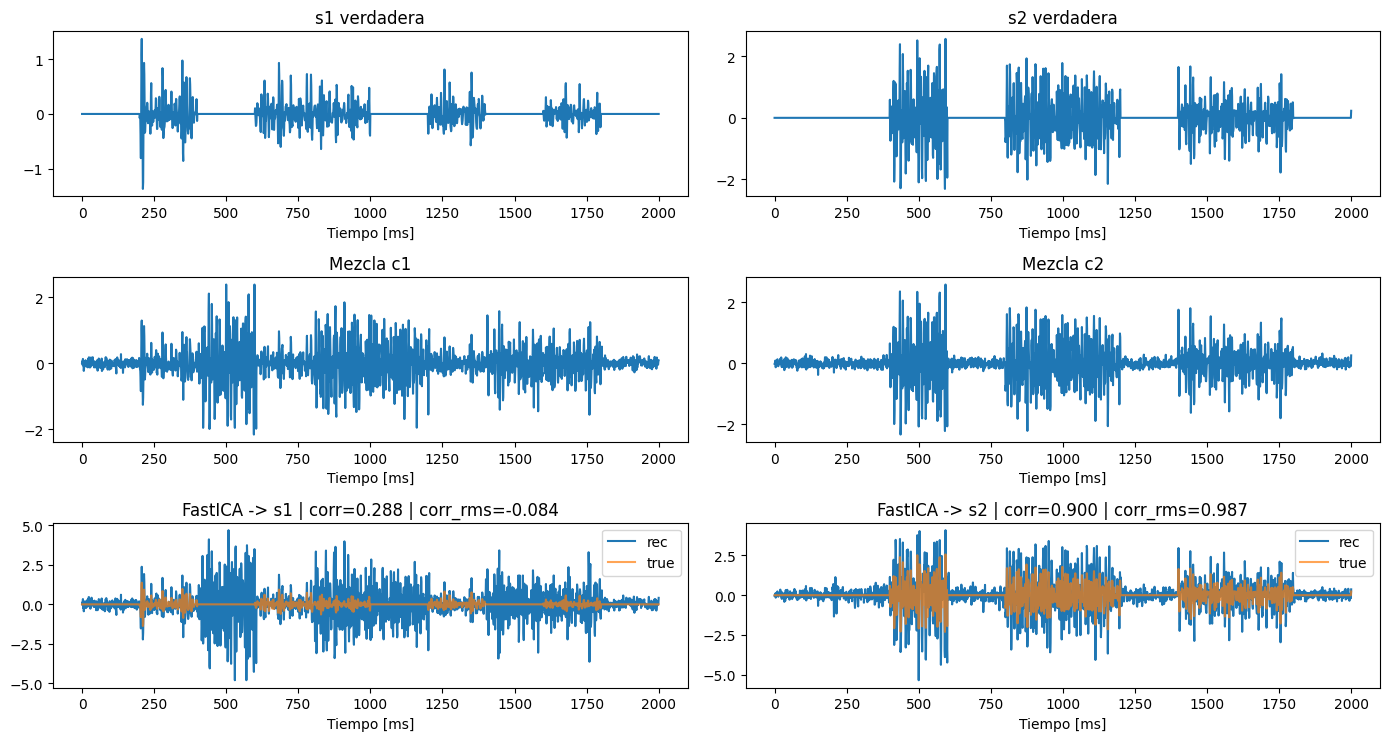
\includegraphics[width=\linewidth]{figuras/ICA/ica_result_noise_delay_09.png}
    }
    \caption{Separation under noisy convolutive mixing. Parameters were set to $\sigma=0.1$, $\beta=0.9$ and $\tau=\qty{5}{ms}$. FastICA now fails to maintain both temporal correlation and activation patterns for $s_1$ due to the significant delayed contribution interference from $s_2$.}
    \label{fig:ica_result_noise_delay09}
\end{figure}

Since the delayed contribution interference is also dependent on $\beta^2$, decreasing the influence of the dominant significantly improve the separation. Figure \ref{fig:ica_result_noise_delay} shows the results of the exact same experiment, but with the $\beta=0.3$. The separation of the target source $s_1$ sees a significant improvement in both temporal and RMS envelope correlations after reducing the value of the $\beta$ parameter.

\begin{figure}[H]
    \centering
    \makebox[\textwidth][c]{%
        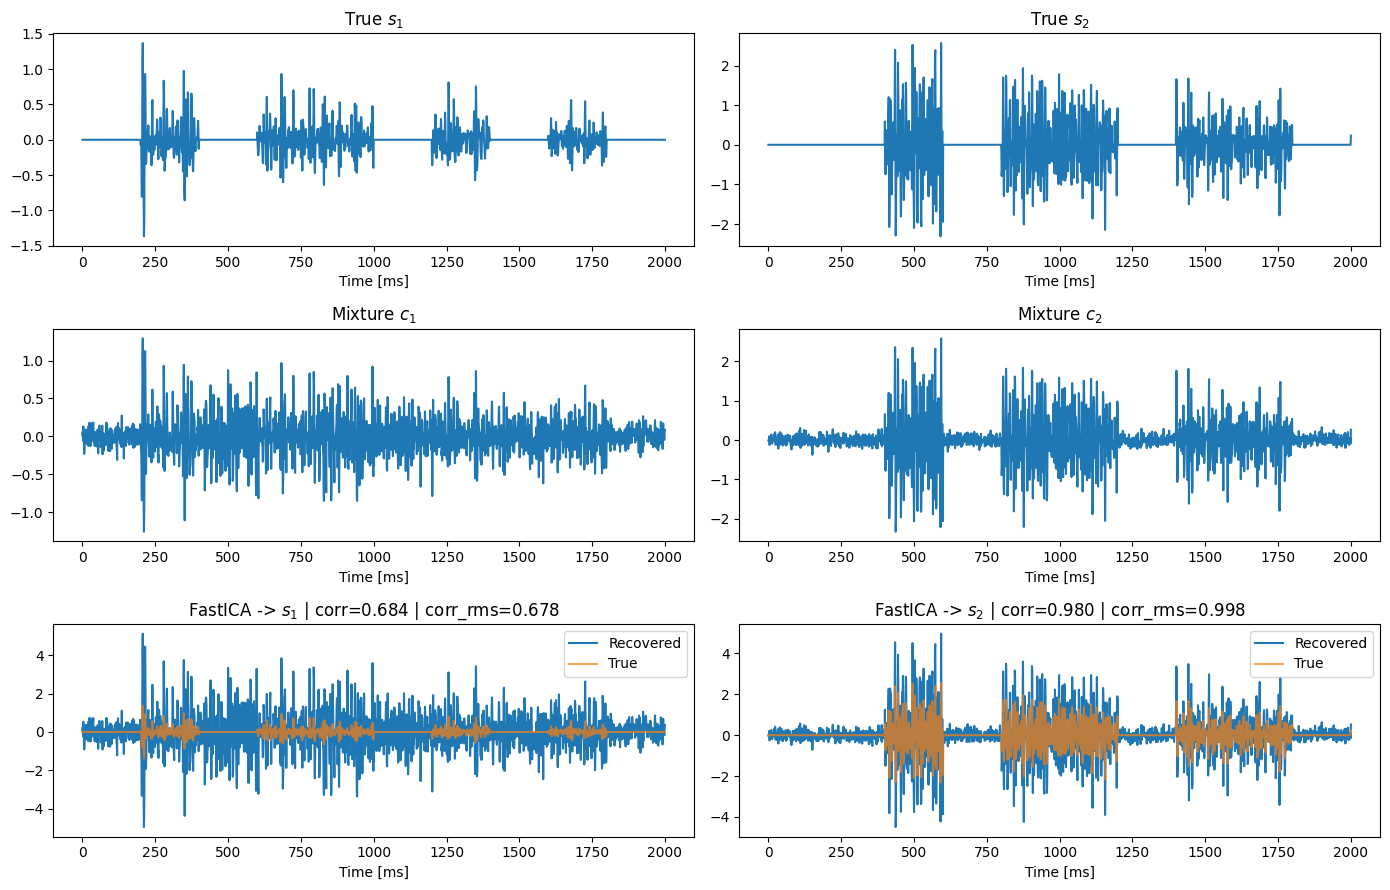
\includegraphics[width=\linewidth,height=9cm]{figuras/ICA/ica_result_noise_delay.png}
    }
    \caption{Separation under noisy convolutive mixing. Parameters were set to $\sigma=0.1$, $\beta=0.3$ and $\tau=\qty{5}{ms}$. FastICA now experiences a smaller delayed contribution interference due to the reduction of the $\beta$ parameter.}
    \label{fig:ica_result_noise_delay}
\end{figure}

One final aspect to consider is that the effect of the delay $\tau$ does not necessarily follow a linear relationship with separation quality. This is because the interference introduced by the delayed contribution (Equation \ref{eq:delay_contamination_term}) depends on the autocorrelation of the interference source at that specific delay $\mathbf{R}_{s2}(\tau)$ . Therefore, the experiments focused on representative delay conditions rather than sweeping isolated delay values.

\subsection{ICA Experiments Conclusion}

ICA results in a considerably effective algorithm for the problem involving the IIT study. However, the algorithm depends mainly on the variances of the EMG signals, which cannot be easily controlled even in a experimental environment. Additionally, temporal delays between channels combined with noise compromise the assumptions of the algorithm, leading to a separation with erroneous activation patterns.

More specifically, ICA is likely to recover $s_1$
in ideal or semi-ideal cases because of the structure of the two-source problem formulation. The algorithm first finds the direction that best optimizes the non-Gaussianity, which is usually aligned with the statistically dominant source $s_2$. Once this direction is identified, the second component is estimated as the remaining orthogonal direction after whitening, which theoretically corresponds to $s_1$. However, when noise and delay become more significant, $s1$ is no longer necessarily aligned to dominant component direction. 
 

In the next chapters, other algorithms will be discussed in other to assess if they can achieve a better performance where ICA fails.